\documentclass[12pt, titlepage]{article}

\usepackage{booktabs}
\usepackage{tabularx}
\usepackage{hyperref}
\usepackage{float}
\usepackage{graphicx}
\hypersetup{
    colorlinks,
    citecolor=black,
    filecolor=black,
    linkcolor=red,
    urlcolor=blue
}
\usepackage[round]{natbib}

\input{../Comments}
%% Common Parts

\newcommand{\progname}{Baja Dynamics} % PUT YOUR PROGRAM NAME HERE
\newcommand{\authname}{Team \#17, Team Name
\\ Grace McKenna
\\ Travis Wing
\\ Cameron Dunn
\\ Kai Arseneau} % AUTHOR NAMES                  

\usepackage{hyperref}
    \hypersetup{colorlinks=true, linkcolor=blue, citecolor=blue, filecolor=blue,
                urlcolor=blue, unicode=false}
    \urlstyle{same}
                                


\begin{document}

\title{Verification and Validation Report: \progname} 
\author{\authname}
\date{\today}
	
\maketitle

\pagenumbering{roman}

\section{Revision History}

\begin{tabularx}{\textwidth}{p{3cm}p{2cm}X}
\toprule {\bf Date} & {\bf Version} & {\bf Notes}\\
\midrule
Date 1 & 1.0 & Notes\\
Date 2 & 1.1 & Notes\\
\bottomrule
\end{tabularx}

~\newpage

\section{Symbols, Abbreviations and Acronyms}

\renewcommand{\arraystretch}{1.2}
\begin{tabular}{l l} 
  \toprule		
  \textbf{symbol} & \textbf{description}\\
  \midrule 
  T & Test\\
  \bottomrule
\end{tabular}\\

\wss{symbols, abbreviations or acronyms -- you can reference the SRS tables if needed}

\newpage

\tableofcontents

\listoftables %if appropriate

\listoffigures %if appropriate

\newpage

\pagenumbering{arabic}

This document ...

\section{Functional Requirements Evaluation}

\section{Nonfunctional Requirements Evaluation}

This section will cover the evaluation of the Nonfunctional Requirements. 

\subsection{Accuracy}
		
\subsection{Usability}
The Usability/Understandability survey remains in progress at this time and results will be discussed in the \href{file:../UsabilityReport/UsabilityReport.pdf}{Usability Report}. 
Therefore, Usability test-1 and Usability test-2 have not been fully completed yet, however as they are in progress these tests will be completed as future work. 

\begin{enumerate}
\item{\textbf{test-1}: Navigating Main Interface}\\
Survey question: On a scale of 1-5 with 1 being extremely difficult and 5 being extremely easy, how easy was it to navigate the main interface? 
\item{\textbf{test-2}: Use of Most Common Features}\\
Survey question: For the following main features: Inputting parameters, Adjusting parameters, Viewing data outputs, Saving and exporting data. 
Rate each feature on a scale of 1-5 with 1 being extremely difficult and 5 being extremely easy
\end{enumerate}

\subsection{Maintainability}
The maintainability tests are designed to test how maintainable the system is given likely future changes.
\begin{enumerate}
\item{\textbf{test-1}: Maintainability}\\
This test was manually completed where the amount of time and number of lines of code
will be recorded when implementing the changes that correspond to the 2023 CVT configuration. 
Implementation of the 2023 CVT parameters takes at most 20 minutes with modifications to appropriately 26 lines of code in the \texttt{car\_specs.py}.
Thus, the system is easily maintainability and the number of lines modified and time taken is minimal given a total change in parameters of the CVT. 
\end{enumerate}
\subsection{Verifiability}

\subsection{Understandability}
The Usability/Understandability survey remains in progress at this time and results will be discussed in the \href{file:../UsabilityReport/UsabilityReport.pdf}{Usability Report}. 
Therefore, Understandability test-1 and Understandability test-2 have not been completed yet, however as they are in progress these tests will completed as future work. 

\begin{enumerate}
  \item{\textbf{test-1}: Function Purpose}\\
  Survey question: For the following main features: Inputting parameters, Adjusting parameters, Viewing data outputs, Saving and exporting data. 
  Was the purpose of each function clear, on a scale of 1-5 with 1 being very unclear and 5 being extremely clear. 
  \item{\textbf{test-2}: Understanding Simulation Outputs}\\
  Survey question: On a scale of 1-5, with 1 being very unclear and 5 being extremely clear, how well did you understand the simulation results and output?
\end{enumerate}

\subsection{Reusability}

The reusability tests are designed to assess how easily the system can be adapted to new or modified configurations. 
\begin{enumerate}
    \item {\textbf{test-1}: Reusability}\\
    This test was manually performed by the teams, where the time taken and number of lines of code modified were recorded when implementing the 2023 CVT configuration. 
    Implementation of the 2023 CVT parameters requires at most 20 minutes and involves modifications to approximately 26 lines of code in the \texttt{car\_specs.py} file. 
    These minimal changes demonstrate the system's high reusability, as it can be quickly adapted to new CVT configurations with little effort and modification.
\end{enumerate}
	
\section{Comparison to Existing Implementation}	

Not applicable for this project.
\section{Unit Testing}

\subsection{Back End Unit Testing}
The back end was fully covered by unit tests except for a several files which were not suited for unit testing as they were mainly constants or did not provide functionality that could be tested. \\
\\
The test structure that was created was to essentially mirror how the codebase is organized. There is a test folder which houses all the tests, then inside that there is a simulations and utils folder which contain mirrored test files of the actual files under src/simulations or src/utils.\\
\\
The tests were written using the built in unittest module in python. The tests were run using the command coverage run -m unittest discover -s test/simulations -s test/utils. This command runs all the tests in those two folders using the coverage library.\\
\\
A coverage report was generated using the command coverage report -m.\\
\\
This command generates a report that shows the percentage of code that was covered by the tests. The report also shows which lines were not covered by the tests.
This can be seen in section 11 of this document.\\

\subsection{Front End Unit Testing}
The front end communication protocol was fully covered by unit tests besides the function that calls the python script since it is dependent on the back end Implementation.
\\
The tests are stored in a separate project within the front end solution. They are written using the MS Unit Testing Framework and are ran using the dotnet test command.
\\
A coverage report was generated using the JetBrains dotCover tool which shows the percentage of code that was covered by the tests.  

\section{Changes Due to Testing}

\wss{This section should highlight how feedback from the users and from 
the supervisor (when one exists) shaped the final product.  In particular 
the feedback from the Rev 0 demo to the supervisor (or to potential users) 
should be highlighted.}

\subsection{Front End Changes}
On the front end, many changes were made to support unit testing. The communication protocol was separated from the main Unity project since Unity was not compatible with the MS Unit Testing Framework.
\\
Moving the communication protocol into a separate project allowed for the simplification of the code base by isolating responsibilities and improving modularization.
\\
There were also changes on the front end to support the requested changes from the Rev 0 demo. The input parameters were updated to be stored in a csv file and read from there.
\\
This changes was to facilitate the implementation of uploading and downloading the parameters from the front end which was a requested feature from the Rev 0 demo.

\section{Automated Testing}
Both back and front end sets of unit tests were automated and added to the CI/CD pipeline. Now whenever there is a commit it must pass all the tess in order to be verified.
If there is an error it will fail and state which tests failed. This is a good way to ensure that the code is always working as expected.\\
\\
As well the back end coverage report is also generated in the CI/CD run so you can see how much of the code is being covered by tests at that moment.
\\
The configuration for the CI/CD can be seen here: \url{https://github.com/gr812b/CVT-Simulator/blob/develop/.github/workflows/ci.yaml}
\section{Trace to Requirements}
		
\section{Trace to Modules}		

\section{Code Coverage Metrics}

\begin{figure}[H]
  \begin{center}
   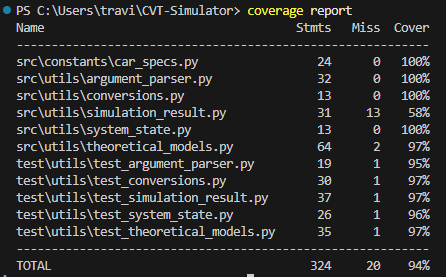
\includegraphics[width=0.7\textwidth]{UnitTestCoverageReport.png}
  \caption{Back End Code Coverage}
  \label{Fig_Home} 
  \end{center}
\end{figure}

\begin{figure}[H]
  \begin{center}
   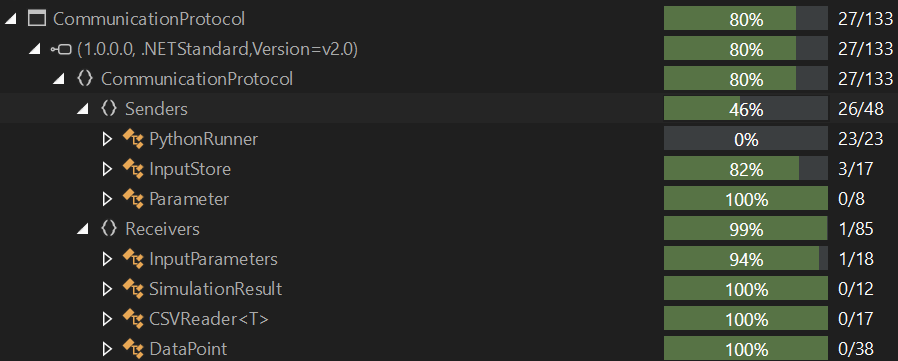
\includegraphics[width=0.7\textwidth]{CSUnitTestCoverage.png}
  \caption{Front End Code Coverage}
  \label{Fig_Home} 
  \end{center}
\end{figure}


\bibliographystyle{plainnat}
\bibliography{../../refs/References}

\newpage{}
\section*{Appendix --- Reflection}

The information in this section will be used to evaluate the team members on the
graduate attribute of Reflection.

\input{../Reflection.tex}

\begin{enumerate}
  \item What went well while writing this deliverable? 
  \item What pain points did you experience during this deliverable, and how
    did you resolve them?
  \item Which parts of this document stemmed from speaking to your client(s) or
  a proxy (e.g. your peers)? Which ones were not, and why?
  \item In what ways was the Verification and Validation (VnV) Plan different
  from the activities that were actually conducted for VnV?  If there were
  differences, what changes required the modification in the plan?  Why did
  these changes occur?  Would you be able to anticipate these changes in future
  projects?  If there weren't any differences, how was your team able to clearly
  predict a feasible amount of effort and the right tasks needed to build the
  evidence that demonstrates the required quality?  (It is expected that most
  teams will have had to deviate from their original VnV Plan.)
\end{enumerate}

\end{document}